% !TEX encoding = UTF-8 Unicode
%!TEX root = thesis.tex
% !TEX spellcheck = en-US
%%=========================================
\chapter{Implementation and Simulation of Sensors}
Using nautical charts, information about other simulated agents and 3D models of installations in sea it is possible to generate realistic sensor data for HIL simulations. This section contains an overview of the implementation of important sensors used on Odin and a brief discussion about how sensor data can be simulated.

\section{Sensors Implemented on Odin}
A brief overview of the sensors on Odin used for situational awareness above the surface should come here.

\subsection{Radar}
...

\newpage
\subsection{Velodyne LiDAR HDL-32E}
\begin{wrapfigure}[14]{l}{0.3\textwidth}
	\vspace{-30pt}
	\begin{center}
		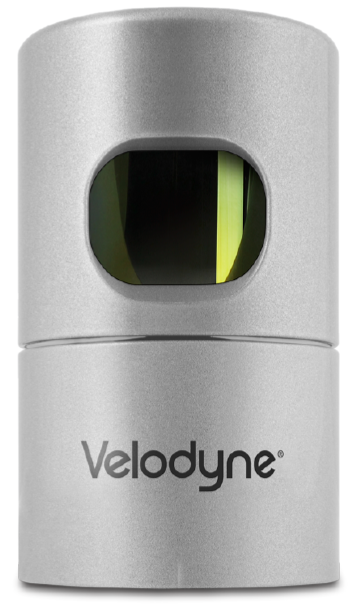
\includegraphics[width= 0.9\linewidth]{fig/VelodyneHDL32Ecase}
		\vspace{-20pt}
		\caption{\it{Velodyne LiDAR HDL-32E used on Odin for above-the-surface 3D analysis.}}
		\label{fig:velodyneCasing}
	\end{center}
	
\end{wrapfigure}
For analysis of the nearby environment above the surface a LiDAR is used to create a 3D point cloud. The model used on Odin is a Velodyne HDL-32E\footnote{Velodyne manual (need reference)} as seen in figure \ref{fig:velodyneCasing}. A LiDAR can measure the distance to points around the sensor by firing a laser and measure the time it takes for the light to return. The distance is then saved along with the horizontal and vertical angle of the laser, so that the positions of the measured points can be used to generate a 3D model of the nearby environment. Velodyne HDL-32E generates 700,000 points per second with $\pm2$cm accuracy at 80m-100m range. The LiDAR spins around the vertical axis to achieve a $360\degree$ horizontal field of view (FOV), and a combination of 32 lasers stacked vertically yields a $40\degree$ vertical FOV ($+10\degree$ to $-30\degree$). An external GPS should be connected to the LiDAR for time pulse synchronization.

Uncalibrated point cloud data packets are transmitted from the LiDAR over a standard ethernet cable using UDP. The packet format is well documented in the user manual so that they should be easy to decompose by a custom made point cloud processing unit. A calibration table must be used for vertical correction for each laser. This table is included on a CD delivered with the HDL-32E.
 


\section{Simulation of Sensor Data from Virtual Environment}
The feasibility of simulating realistic sensor data from a virtual environment will be discussed in this section, as well as complexity and benefits regarding simulation of raw versus preprocessed sensor data. Information, hardware and software needed to generate data from each sensor will be also be discussed.

\subsection{Simulating Data from Radar}
...

\subsection{Simulating Data from LiDAR}
The protocol of the data transfer from Velodyne HDL-32E is well documented. Given a 3D model of the surrounding environment with easy access to angle and distance calculations it should be feasible to generate a realistic point cloud. The point cloud can be represented as data packets using the HDL-32E protocol and sent over ethernet to the interface between HIL simulator and the control system. This way it would be possible to simulate raw sensor readings from the HDL-32E. This is assumed to be beneficial to the developers of the simulated vehicle as a larger chain of HW/SW can be tested in the simulated environment.

- Should the GPS used for clock synchronization also be simulated or could we use the one on the vehicle being tested?



\subsection{Raw vs Preprocessed Sensor Data}
Complexity and benefits regarding generating raw data versus preprocessed information.







